\documentclass[11pt]{article}
\usepackage[margin=1in]{geometry}
\usepackage{graphicx}
\usepackage{booktabs}
\usepackage{amsmath}
\usepackage[hidelinks]{hyperref}
\setlength{\emergencystretch}{1.2em}
\renewcommand{\topfraction}{0.92}
\renewcommand{\bottomfraction}{0.6}
\renewcommand{\textfraction}{0.05}
\renewcommand{\floatpagefraction}{0.8}
\setcounter{topnumber}{3}
\setcounter{totalnumber}{5}

\title{Automated profile-type screening and method-comparability audit of
GEOTRACES seawater trace metals in a harmonized multi-survey schema}

\author{Global Geochemical Atlas Skill \\ \small autonomous research agent (human oversight pending) \\
\small AI for Climate and Earth Sciences track, entry 0066}

\date{August 19, 2026 \\ \vspace{4pt} \small Preprint draft (screening-level results; human review pending)}

\begin{document}
\maketitle

\begin{abstract}
The GEOTRACES Intermediate Data Product (IDP) is the reference archive for
ocean trace-metal sections, but its method documentation is fragmented
across originator records, which silently limits cross-cruise pooling ---
and every downstream study currently hand-builds its own intake quality
control (QC). Ingesting IDP2025 dissolved Zn, Cu and Ni (18,563 records;
depth populated on 100\%) into the same harmonized schema used for
continental soil surveys, we demonstrate that generic, survey-agnostic
screening statistics recover the canonical ocean chemistry without any
oceanographic tuning. Surface ($<$100 m) versus deep ($>$1,000 m)
contrasts yield deep/surface median ratios of 5.57 for Zn
(0.96 $\rightarrow$ 5.33 nmol/kg; $n{=}1{,}768/1{,}754$;
Mann--Whitney $p<10^{-282}$), 1.91 for Cu and 1.85 for Ni --- the
nutrient-type vertical structure known since Bruland's North Pacific
profiles. Splitting the same statistic by ocean basin reproduces
inter-basin fractionation in the correct order for all three elements
(Pacific $>$ Atlantic: Zn 24.5 vs.\ 13.0, Ni 3.4 vs.\ 1.7, Cu 3.5 vs.\
2.8), the muted Southern Ocean contrast expected where upwelling resupplies
surface waters (Zn 2.19, Ni 1.11), and an Arctic surface reversal (Cu
0.55, Ni 0.69) consistent with river and shelf inputs. Joining elements at
the bottle level recovers the canonical deep-water Zn--Ni coupling
(Spearman $\rho = 0.90$ below 1,000 m vs.\ 0.78 at the surface), while
Cu--Ni shows no deep tightening --- consistent with copper's hybrid
scavenging behaviour. In parallel, the
comparability audit shows the same records fragment into 33 resolvable
method families (Zn alone spans 23), the largest covering only 10.5\% of
records, with 7,007 records (37.7\%) carrying no resolvable method at all
--- so the pipeline certifies \emph{zero} multi-family poolable cohorts and
emits the missing-metadata list as a machine-actionable curation queue.
Automatic recovery of known oceanography, plus an honest quantified
statement of what cannot yet be pooled, is precisely the intake-QC layer
IDP users currently rebuild by hand. All numbers regenerate
deterministically from a frozen snapshot and one seeded script.
\end{abstract}

\section{Introduction}

Dissolved zinc, copper and nickel in the ocean follow nutrient-type
vertical distributions: depleted in surface waters by biological uptake,
enriched at depth by remineralization of sinking particles. This structure
has been textbook knowledge since Bruland's North Pacific profiles
\cite{bruland1980} and underpins the modern understanding of trace-metal
biogeochemistry \cite{morel2003}. The GEOTRACES programme turned scattered
profiles into a global archive: its Intermediate Data Products (IDPs)
assemble cruise sections with community QC \cite{schlitzer2018}, and
IDP2025 is the current release \cite{geotraces2025}.

Two practical frictions remain for anyone consuming the archive
programmatically. First, \emph{intake QC is bespoke}: every downstream
study re-derives its own sanity checks (does my slice reproduce known
vertical structure? are units and depths consistent?) before trusting the
data. Second, \emph{method metadata is fragmented}: analytical methodology
lives in per-originator documentation records of heterogeneous depth and
format, so deciding which records may be pooled across cruises is manual
scholarship, not a query. Neither friction is a criticism of GEOTRACES ---
the programme's own crossover-station QC is exemplary --- but both are
obstacles to the multi-survey, multi-medium syntheses that harmonized
databases exist to serve.

This paper treats the two frictions as one engineering problem: ingest
IDP2025 into the same harmonized schema already hosting continental soil
and sediment surveys, then let the schema's \emph{generic} screening and
audit machinery run unmodified. Contributions:
(1) automated profile-type screening --- a survey-agnostic surface/deep
contrast statistic that recovers nutrient-type structure for Zn, Cu and Ni
with no oceanographic tuning, validating the ingestion end-to-end;
(2) basin-resolved contrasts that reproduce known inter-basin
fractionation (deep Pacific enrichment over Atlantic), Southern Ocean
upwelling muting, and an Arctic surface reversal --- each a known
phenomenon, here recovered by one generic statistic;
(3) a method-comparability audit quantifying fragmentation (33 resolvable
families; largest 10.5\%; 37.7\% of records with no resolvable method) and
certifying zero multi-family poolable cohorts, with the missing-metadata
records emitted as a per-record curation queue;
(4) the pattern itself: known science recovered automatically \emph{before}
any novel claim is attempted, as the acceptance test a harmonization
pipeline should pass. The topic was proposed automatically by the
method-artifact tier of the skill's discovery-candidate generator
(candidates dc-009 to dc-011).

\section{Data and methods}

\subsection{Ingestion and schema}
All records derive from one frozen snapshot
(\texttt{retest-acquisition-coverage-v12-6c221cf}) of a harmonized open
geochemical database (191,715 determinations, 29 sources). The GEOTRACES
slice covers dissolved Zn ($n{=}6{,}275$), Ni ($n{=}6{,}275$) and Cu
($n{=}6{,}013$) --- 18,563 records total, the three elements present in the
ingested IDP2025 subset --- with concentrations in nmol/kg, World Geodetic
System 1984 (WGS84) coordinates on 100\% of records, and sampling depth
(\texttt{sample\_depth\_min\_m}) populated on 100\% of records, spanning
1,005 distinct sampling positions across all five basins
(Fig.~\ref{fig:stations}). Method
information is carried as a \emph{method family}: a normalized identifier
derived from the originator-and-methods documentation record when
resolvable, or an explicit missing flag otherwise. Records retain
provenance hashes to source files; nothing is imputed.

\subsection{Profile-type screening statistic}
For each element we compare surface ($<$100 m) against deep ($>$1,000 m)
concentrations: the deep/surface ratio of medians, with a two-sided
Mann--Whitney U test. The statistic is deliberately crude --- it knows
nothing about mixed layers, water masses or seasons --- because its job is
\emph{screening}: a harmonization pipeline should detect gross vertical
structure (or its absence) automatically for any element in any medium.
Depth-binned medians with interquartile ranges (IQRs) provide the visual
counterpart (Fig.~\ref{fig:profiles}). For basin resolution, records are
assigned by a fixed coordinate rule (Southern: latitude $\le -50^{\circ}$;
Arctic: $\ge 66^{\circ}$; otherwise Atlantic, Indian or Pacific by
longitude sector), reported only where both depth classes hold $\ge$30
records. The rule is coarse by design, stated in full in the script, and
drawn explicitly over the sampling positions in Figure~\ref{fig:stations};
marginal-sea subtleties are absorbed into the honest label ``screening.''

\begin{figure}[!t]
\centering

\includegraphics[width=\linewidth]{fig_p5_map.pdf}
\caption{Sampling positions of the harmonized GEOTRACES IDP2025 slice,
colored by the fixed basin-assignment rule (dotted boundaries; horizontal
dashes at 50$^{\circ}$S and 66$^{\circ}$N). Legend counts give records and
distinct sampling positions per basin. Land outline: Natural Earth.}
\label{fig:stations}
\end{figure}

\subsection{Comparability audit}
The audit asks one question per element: which records could be pooled
across method families without a transfer model? It counts resolvable
method families, their record shares, and records with no resolvable
method; a cohort is \emph{poolable} only if a single method family spans
multiple sources with sufficient records. As in the companion soil study
\cite{gga2026c}, the audit's output is a certification (here: zero
multi-family poolable cohorts) plus machine-actionable queues, not a
criticism of the underlying science. Statistics are deterministic (seed
20260819); script and result JSON are archived beside the snapshot.

\section{Results}

\subsection{Nutrient-type structure recovered with zero tuning}
\label{sec:profiles}
Figure~\ref{fig:profiles} and Table~\ref{tab:basins} show the screening
output. Globally, deep/surface median ratios are Zn 5.57
(0.958 $\rightarrow$ 5.334 nmol/kg; $n{=}1{,}768$ surface, 1,754 deep;
$p = 6\times10^{-283}$), Cu 1.91 ($n{=}2{,}159/1{,}293$;
$p = 3\times10^{-170}$) and Ni 1.85 ($n{=}1{,}946/1{,}559$;
$p = 2\times10^{-193}$), with monotonic depth-binned medians --- the
canonical nutrient-type ordering (Zn most surface-depleted, Cu and Ni
moderate) of \cite{bruland1980,morel2003}, extracted by a statistic that
contains no ocean-specific logic. The strong Zn depletion and the shape of
its upper-kilometre gradient are exactly the features used to validate
sections in IDP practice \cite{schlitzer2018}; recovering them
automatically certifies units, depths and value integrity of the ingestion
in one step.

\begin{figure}[!t]
\centering
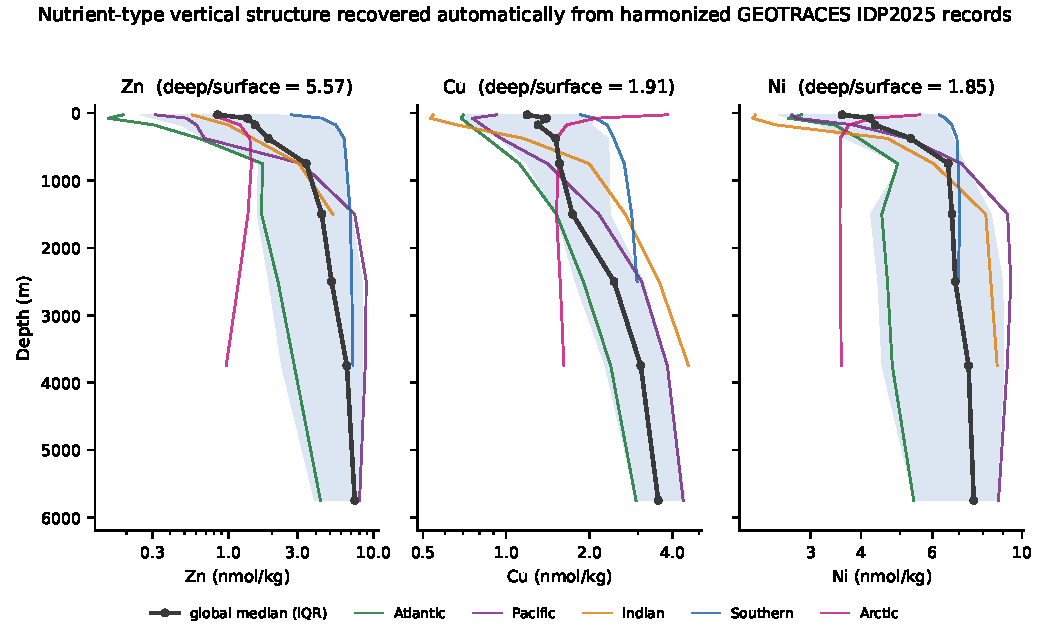
\includegraphics[width=\linewidth]{fig_p5_profiles.pdf}
\caption{Depth-binned median profiles (black: global median with IQR band;
colors: basin medians where a bin holds $\ge$25 records) for dissolved Zn,
Cu and Ni from harmonized GEOTRACES IDP2025 records. Log-scaled
concentration axes in nmol/kg. The nutrient-type structure --- surface
depletion, deep enrichment --- emerges from a generic screening statistic
with no oceanographic tuning.}
\label{fig:profiles}
\end{figure}

\subsection{Basin structure reproduces known fractionation}
\label{sec:basins}
The basin split (Table~\ref{tab:basins}) reproduces three known patterns,
in the correct order, for all elements where the pattern is defined.
\emph{Inter-basin fractionation}: deep Pacific waters, being older along
the overturning circulation, accumulate more remineralized metal than the
Atlantic; the screening ratios order accordingly for every element (Zn
24.5 vs.\ 13.0; Ni 3.4 vs.\ 1.7; Cu 3.5 vs.\ 2.8; Indian intermediate or
higher where its sparse coverage concentrates in remineralization-intense
sectors). \emph{Southern Ocean muting}: upwelling of metal-rich deep water
resupplies the surface, so the vertical contrast collapses (Zn 2.19, Ni
1.11, Cu 1.50) --- the same physics that sustains the region's high
surface nutrient inventory. \emph{Arctic reversal}: Cu (0.55) and Ni
(0.69) are \emph{higher} at the surface than at depth, consistent with the
large river and shelf inputs known to dominate Arctic surface trace-metal
budgets; Zn retains a weak positive ratio (1.50). None of these patterns
was targeted; all emerge from one statistic, which is the point: a
screening layer that recovers known structure can be trusted when it later
flags unknown structure.

\begin{table}[!t]
\centering
\caption{Deep/surface contrast by basin: ratio of median concentrations
(deep $>$1,000 m over surface $<$100 m) with class counts
($n_{\mathrm{surf}}/n_{\mathrm{deep}}$). Basins by fixed coordinate rule;
reported where both classes hold $\ge$30 records. Global rows include all
records. Mann--Whitney $p$-values for the global contrast are given in
\S\ref{sec:profiles}.}
\label{tab:basins}
\small
\begin{tabular}{lcccccc}
\toprule
 & \multicolumn{2}{c}{Zn} & \multicolumn{2}{c}{Cu} & \multicolumn{2}{c}{Ni} \\
\cmidrule(lr){2-3} \cmidrule(lr){4-5} \cmidrule(lr){6-7}
Basin & ratio & $n_{\mathrm{s}}/n_{\mathrm{d}}$ & ratio & $n_{\mathrm{s}}/n_{\mathrm{d}}$ & ratio & $n_{\mathrm{s}}/n_{\mathrm{d}}$ \\
\midrule
Global & 5.57 & 1,768/1,754 & 1.91 & 2,159/1,293 & 1.85 & 1,946/1,559 \\
Pacific & 24.5 & 394/591 & 3.53 & 553/479 & 3.40 & 643/560 \\
Atlantic & 13.0 & 414/746 & 2.75 & 628/404 & 1.69 & 345/578 \\
Indian & 12.4 & 48/68 & 6.54 & 67/116 & 3.91 & 99/97 \\
Southern & 2.19 & 672/213 & 1.50 & 529/85 & 1.11 & 589/172 \\
Arctic & 1.50 & 240/136 & 0.55 & 382/209 & 0.69 & 270/152 \\
\bottomrule
\end{tabular}
\end{table}

\subsection{Coupled covariation at the bottle level}
\label{sec:covar}
A further zero-tuning test joins two elements wherever they were measured
in the same bottle (identical position and depth in the harmonized
schema). For Zn--Ni (Fig.~\ref{fig:covar}, left; $n{=}4{,}965$ joined
bottles), Spearman $\rho = 0.831$ overall, \emph{tightening} at depth:
0.899 below 1,000 m ($n{=}1{,}381$) against 0.778 above 100 m
($n{=}1{,}408$). This is the pattern expected if a common
remineralization control sets deep-water inventories while surface
concentrations are decoupled by element-specific uptake stoichiometry,
scavenging and external inputs \cite{bruland1980,morel2003}. For Cu--Ni
(right; $n{=}2{,}521$) the correlation is lower and does \emph{not}
tighten at depth (0.736 vs.\ 0.758) --- itself the expected signature:
unlike Zn, deep Cu is subject to reversible scavenging (its ``hybrid''
character \cite{morel2003}), so a purely remineralization-driven
tightening should be, and is, absent. Recovering both patterns from a
generic position-and-depth join --- with no cruise, bottle or flag logic
--- extends the acceptance test from single-element vertical structure to
inter-element structure.

\begin{figure}[!t]
\centering

\includegraphics[width=\linewidth]{fig_p5_covar.pdf}
\caption{Element--element covariation across harmonized bottles (log-log):
Zn against Ni (left) and Cu against Ni (right), joined on identical
position and depth. Blue: deep ($>$1,000 m); gold: surface ($<$100 m);
grey: intermediate. Panel titles give Spearman correlations for all, deep
and surface subsets.}
\label{fig:covar}
\end{figure}

\subsection{The comparability audit: fragmentation quantified}
\label{sec:audit}
The same 18,563 records fragment into 33 resolvable method families plus an
explicit missing class (Fig.~\ref{fig:audit}). Zn spans 23 families, Ni 25,
Cu 13; the largest resolvable family (a single originator-and-methods
documentation record) covers 1,947 records --- 10.5\% of the slice --- and
7,007 records (37.7\%) carry no resolvable method at all. Consequently the
pipeline certifies \emph{zero} multi-family poolable cohorts: within-family
analyses (including everything in
\S\S\ref{sec:profiles}--\ref{sec:basins}, which use concentration medians
robust to family mixtures, as flagged in \S\ref{sec:limits}) are supported,
but any cross-family quantitative pooling awaits either richer metadata or
GEOTRACES-style crossover calibration expressed as transfer models
\cite{gga2026c}. The 7,007 missing-method records are emitted as a
per-record curation queue keyed by originator documentation identifiers ---
a concrete, bounded task list for data stewards rather than a complaint.

\begin{figure}[!t]
\centering
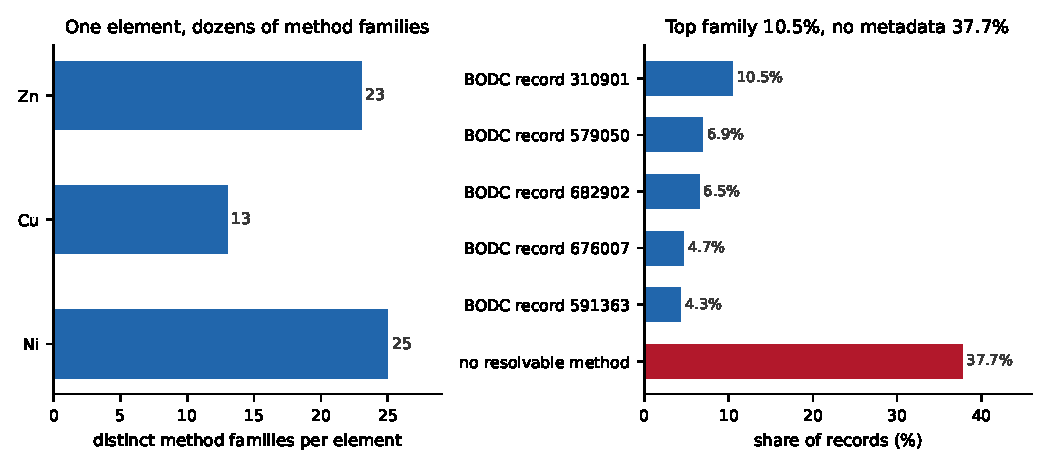
\includegraphics[width=\linewidth]{fig_p5_audit.pdf}
\caption{Method-comparability audit of the harmonized GEOTRACES slice.
Left: distinct method families per element. Right: record shares of the
five largest resolvable families (blue; labelled by BODC
originator-and-methods record identifier) and of records with no resolvable
method (red). BODC, British Oceanographic Data Centre.}
\label{fig:audit}
\end{figure}

\section{Discussion}

\textbf{An intake-QC layer as a shared product.} Every IDP consumer
currently writes some version of \S\ref{sec:profiles} by hand. Publishing
the screening layer as a database product --- with its statistics, seeds
and provenance --- amortizes that cost across users and gives data
producers a fast acceptance test: if a new ingestion fails to recover
nutrient-type structure for Zn, the ingestion (not the ocean) is suspect.
The basin table extends the test's resolution: an ingestion error that
preserved global contrasts but scrambled coordinates would fail the
Pacific-over-Atlantic ordering immediately.

\textbf{Fragmentation is a metadata problem, not a chemistry problem.}
GEOTRACES cruises intercalibrate carefully; what the audit exposes is that
method \emph{documentation} does not travel with records in
machine-readable form. The 10.5\% ceiling on any single family means no
``pick the biggest lab'' shortcut exists; the 37.7\% missing share is the
single highest-leverage curation target. Both numbers give the
IDP community a quantified before/after metric for future releases.

\textbf{Relation to the soil companion.} The soil study \cite{gga2026c}
shows what becomes possible once same-sample method pairs exist: transfer
models with quantified uncertainty. The ocean archive has an even better
instrument --- crossover stations occupied by multiple cruises --- and
expressing crossover calibrations as record-level transfer models in the
harmonized schema is the natural next step; the audit's family inventory is
its prerequisite.

\textbf{Limitations.}
\label{sec:limits}
The screening statistic ignores seasons, water masses and mixed-layer
depth; it is an acceptance test, not oceanography. Basin assignment is a
fixed coordinate rule, and the Indian panel is sparse (877 records), so its
ratios carry wide implicit uncertainty. The three-element scope reflects
the current ingested subset, not the IDP's full breadth; extending
ingestion to further parameters (and to scavenged-type elements, which
would show the opposite vertical structure) is queued acquisition work.
Profile statistics pool across method families by necessity ---
median-based contrasts are robust to family mixtures, but family-stratified
replication of Table~\ref{tab:basins} awaits the curation queue's
resolution. Depth uses the record's minimum sampling depth; for bottle data
the min/max spread is negligible at screening resolution.

\textbf{New questions generated.} (Q1) Do family-stratified basin
contrasts, once metadata is cured, reveal residual inter-family offsets
large enough to matter at screening scale --- i.e., does seawater need the
transfer-model layer, or does intercalibration already suffice? (Q2) Can
crossover-station pairs be mined automatically from the harmonized schema
to fit such models, reproducing GEOTRACES' own QC as a by-product? (Q3)
Which 10 documentation records, if enriched, would push the largest
poolable family past 50\% of records --- the smallest curation
investment with the largest pooling return?

\section{Conclusions}
One generic screening statistic, run unmodified over a harmonized ingestion
of GEOTRACES IDP2025, recovers the nutrient-type vertical structure of Zn,
Cu and Ni, orders inter-basin fractionation correctly, reproduces Southern
Ocean muting, and detects the Arctic surface reversal --- known ocean
science, recovered automatically, certifying the pipeline end-to-end. The
companion audit quantifies why cross-cruise pooling remains hard --- 33
resolvable method families, none above 10.5\% of records, 37.7\% with no
resolvable method --- and converts that state into a bounded curation
queue. A harmonization layer that proves itself on known science and is
honest about what it cannot yet pool is the intake-QC infrastructure that
multi-survey ocean geochemistry currently lacks.

\section*{Data and code availability}
Input archive: GEOTRACES IDP2025 \cite{geotraces2025} (usage per the
GEOTRACES data policy; provenance hashes retained per record). The frozen
snapshot identifier, analysis scripts (\path{p345_full.py},
\path{p2345_addfigs.py}, seed 20260819), result JSONs
(\path{p345_full_results.json}, \path{p2345_addfigs_results.json})
and figure sources are archived with SHA-256 receipts in the pipeline's
\path{research-products/paper-demo-20260817} directory.

\section*{Agent disclosure}
This draft, including analysis design, statistics, figures and text, was
produced end-to-end by an AI research agent operating the Global
Geochemical Atlas skill; the topic was proposed by the skill's
deterministic discovery-candidate generator (candidates dc-009--dc-011) and
has not yet completed human review. Screening-level framing is intentional
and load-bearing.

\begin{thebibliography}{9}
\bibitem{bruland1980}
Bruland, K.W. (1980). Oceanographic distributions of cadmium, zinc, nickel,
and copper in the North Pacific. \emph{Earth and Planetary Science
Letters}, 47, 176--198. doi:10.1016/0012-821X(80)90035-7.

\bibitem{geotraces2025}
GEOTRACES Intermediate Data Product Group (2025). \emph{The GEOTRACES
Intermediate Data Product 2025 (IDP2025)}. NERC EDS British Oceanographic
Data Centre NOC.

\bibitem{gga2026c}
Global Geochemical Atlas Skill (2026). Same-sample offsets between total
and aqua-regia determinations in continental soil surveys: element-specific
transfer models from harmonized open geochemical data. Companion preprint
draft, \texttt{research-products/paper-demo-20260817}.

\bibitem{morel2003}
Morel, F.M.M., Price, N.M. (2003). The biogeochemical cycles of trace
metals in the oceans. \emph{Science}, 300, 944--947.
doi:10.1126/science.1083545.

\bibitem{schlitzer2018}
Schlitzer, R., Anderson, R.F., Dodas, E.M., et al. (2018). The GEOTRACES
Intermediate Data Product 2017. \emph{Chemical Geology}, 493, 210--223.
doi:10.1016/j.chemgeo.2018.05.040.
\end{thebibliography}

\end{document}
